% Options for packages loaded elsewhere
\PassOptionsToPackage{unicode}{hyperref}
\PassOptionsToPackage{hyphens}{url}
%
\documentclass[
]{article}
\usepackage{amsmath,amssymb}
\usepackage{lmodern}
\usepackage{iftex}
\ifPDFTeX
  \usepackage[T1]{fontenc}
  \usepackage[utf8]{inputenc}
  \usepackage{textcomp} % provide euro and other symbols
\else % if luatex or xetex
  \usepackage{unicode-math}
  \defaultfontfeatures{Scale=MatchLowercase}
  \defaultfontfeatures[\rmfamily]{Ligatures=TeX,Scale=1}
\fi
% Use upquote if available, for straight quotes in verbatim environments
\IfFileExists{upquote.sty}{\usepackage{upquote}}{}
\IfFileExists{microtype.sty}{% use microtype if available
  \usepackage[]{microtype}
  \UseMicrotypeSet[protrusion]{basicmath} % disable protrusion for tt fonts
}{}
\makeatletter
\@ifundefined{KOMAClassName}{% if non-KOMA class
  \IfFileExists{parskip.sty}{%
    \usepackage{parskip}
  }{% else
    \setlength{\parindent}{0pt}
    \setlength{\parskip}{6pt plus 2pt minus 1pt}}
}{% if KOMA class
  \KOMAoptions{parskip=half}}
\makeatother
\usepackage{xcolor}
\usepackage[margin=1in]{geometry}
\usepackage{color}
\usepackage{fancyvrb}
\newcommand{\VerbBar}{|}
\newcommand{\VERB}{\Verb[commandchars=\\\{\}]}
\DefineVerbatimEnvironment{Highlighting}{Verbatim}{commandchars=\\\{\}}
% Add ',fontsize=\small' for more characters per line
\usepackage{framed}
\definecolor{shadecolor}{RGB}{248,248,248}
\newenvironment{Shaded}{\begin{snugshade}}{\end{snugshade}}
\newcommand{\AlertTok}[1]{\textcolor[rgb]{0.94,0.16,0.16}{#1}}
\newcommand{\AnnotationTok}[1]{\textcolor[rgb]{0.56,0.35,0.01}{\textbf{\textit{#1}}}}
\newcommand{\AttributeTok}[1]{\textcolor[rgb]{0.77,0.63,0.00}{#1}}
\newcommand{\BaseNTok}[1]{\textcolor[rgb]{0.00,0.00,0.81}{#1}}
\newcommand{\BuiltInTok}[1]{#1}
\newcommand{\CharTok}[1]{\textcolor[rgb]{0.31,0.60,0.02}{#1}}
\newcommand{\CommentTok}[1]{\textcolor[rgb]{0.56,0.35,0.01}{\textit{#1}}}
\newcommand{\CommentVarTok}[1]{\textcolor[rgb]{0.56,0.35,0.01}{\textbf{\textit{#1}}}}
\newcommand{\ConstantTok}[1]{\textcolor[rgb]{0.00,0.00,0.00}{#1}}
\newcommand{\ControlFlowTok}[1]{\textcolor[rgb]{0.13,0.29,0.53}{\textbf{#1}}}
\newcommand{\DataTypeTok}[1]{\textcolor[rgb]{0.13,0.29,0.53}{#1}}
\newcommand{\DecValTok}[1]{\textcolor[rgb]{0.00,0.00,0.81}{#1}}
\newcommand{\DocumentationTok}[1]{\textcolor[rgb]{0.56,0.35,0.01}{\textbf{\textit{#1}}}}
\newcommand{\ErrorTok}[1]{\textcolor[rgb]{0.64,0.00,0.00}{\textbf{#1}}}
\newcommand{\ExtensionTok}[1]{#1}
\newcommand{\FloatTok}[1]{\textcolor[rgb]{0.00,0.00,0.81}{#1}}
\newcommand{\FunctionTok}[1]{\textcolor[rgb]{0.00,0.00,0.00}{#1}}
\newcommand{\ImportTok}[1]{#1}
\newcommand{\InformationTok}[1]{\textcolor[rgb]{0.56,0.35,0.01}{\textbf{\textit{#1}}}}
\newcommand{\KeywordTok}[1]{\textcolor[rgb]{0.13,0.29,0.53}{\textbf{#1}}}
\newcommand{\NormalTok}[1]{#1}
\newcommand{\OperatorTok}[1]{\textcolor[rgb]{0.81,0.36,0.00}{\textbf{#1}}}
\newcommand{\OtherTok}[1]{\textcolor[rgb]{0.56,0.35,0.01}{#1}}
\newcommand{\PreprocessorTok}[1]{\textcolor[rgb]{0.56,0.35,0.01}{\textit{#1}}}
\newcommand{\RegionMarkerTok}[1]{#1}
\newcommand{\SpecialCharTok}[1]{\textcolor[rgb]{0.00,0.00,0.00}{#1}}
\newcommand{\SpecialStringTok}[1]{\textcolor[rgb]{0.31,0.60,0.02}{#1}}
\newcommand{\StringTok}[1]{\textcolor[rgb]{0.31,0.60,0.02}{#1}}
\newcommand{\VariableTok}[1]{\textcolor[rgb]{0.00,0.00,0.00}{#1}}
\newcommand{\VerbatimStringTok}[1]{\textcolor[rgb]{0.31,0.60,0.02}{#1}}
\newcommand{\WarningTok}[1]{\textcolor[rgb]{0.56,0.35,0.01}{\textbf{\textit{#1}}}}
\usepackage{graphicx}
\makeatletter
\def\maxwidth{\ifdim\Gin@nat@width>\linewidth\linewidth\else\Gin@nat@width\fi}
\def\maxheight{\ifdim\Gin@nat@height>\textheight\textheight\else\Gin@nat@height\fi}
\makeatother
% Scale images if necessary, so that they will not overflow the page
% margins by default, and it is still possible to overwrite the defaults
% using explicit options in \includegraphics[width, height, ...]{}
\setkeys{Gin}{width=\maxwidth,height=\maxheight,keepaspectratio}
% Set default figure placement to htbp
\makeatletter
\def\fps@figure{htbp}
\makeatother
\setlength{\emergencystretch}{3em} % prevent overfull lines
\providecommand{\tightlist}{%
  \setlength{\itemsep}{0pt}\setlength{\parskip}{0pt}}
\setcounter{secnumdepth}{-\maxdimen} % remove section numbering
\ifLuaTeX
  \usepackage{selnolig}  % disable illegal ligatures
\fi
\IfFileExists{bookmark.sty}{\usepackage{bookmark}}{\usepackage{hyperref}}
\IfFileExists{xurl.sty}{\usepackage{xurl}}{} % add URL line breaks if available
\urlstyle{same} % disable monospaced font for URLs
\hypersetup{
  pdftitle={Final Assignment: Reproducing Excel Figures in R},
  pdfauthor={Emily K. Power},
  hidelinks,
  pdfcreator={LaTeX via pandoc}}

\title{Final Assignment: Reproducing Excel Figures in R}
\author{Emily K. Power}
\date{2023-02-02}

\begin{document}
\maketitle

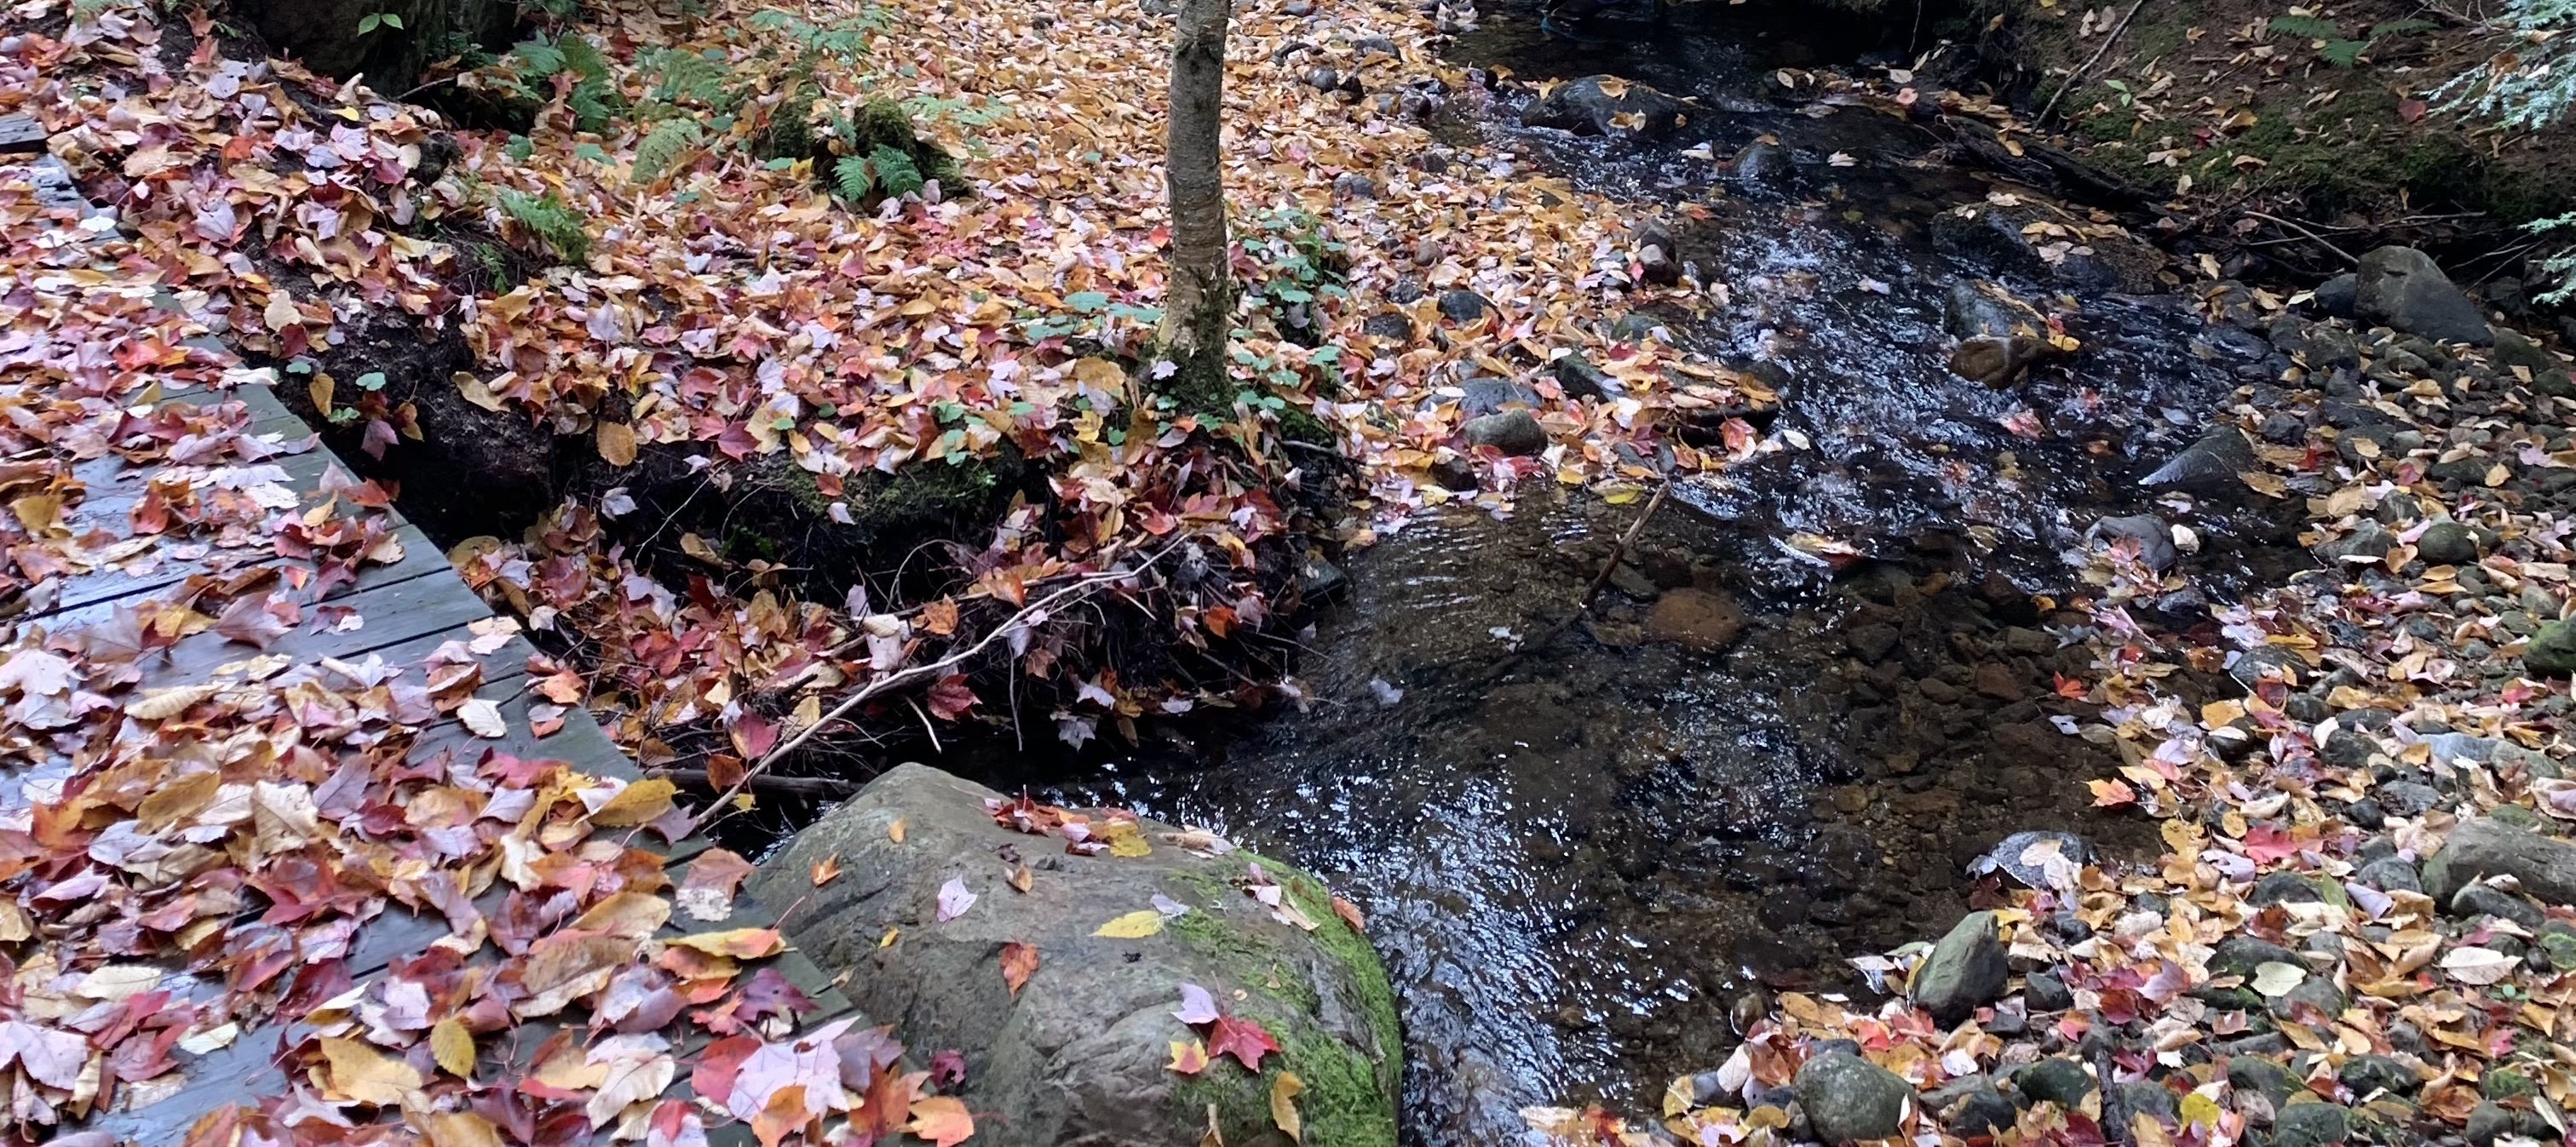
\includegraphics{/Users/emilypower/Desktop/BIOL_1007A/Images/IMG_3102.jpg}

\textbf{For my final assignment, I chose to reproduce some of the
figures that I made this past fall in my Aquatic Ecology course} 🐟🌿

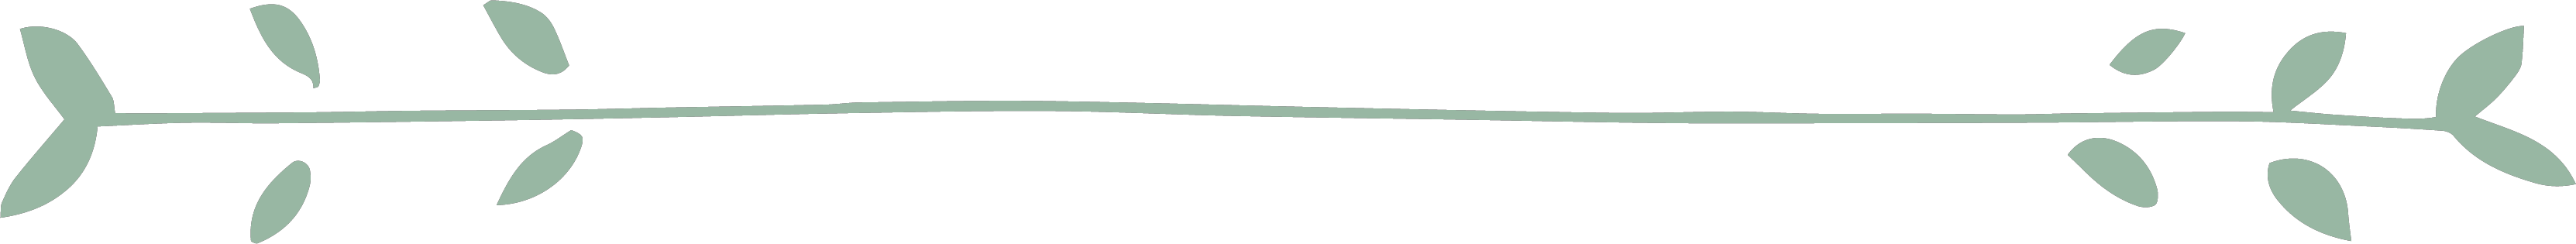
\includegraphics{/Users/emilypower/Desktop/BIOL_1007A/Images/Page_Break_Graphic_D2460FF10315A.png}

Back in October, we conducted research over the course of a few weeks to
investigate the impacts of ski development across lotic ecosystems.

\begin{itemize}
\item
  To do so, we chose two streams that we expected to be impacted by ski
  development (the stream beside the parking lot of the Snowbowl and the
  portion of Brandy Brook that runs through Rikert) to compare to a
  nearby reference stream, Sparks Brook, that we considered to be
  virtually unaffected by ski infrastructure.
\item
  Research included collecting data on stream chemistry, tree canopy
  cover, and water temperature and absorbency.
\item
  \textbf{We also conducted benthic invertebrate sampling to investigate
  if there were any differences in species assemblages between the
  sites.}\\
  \includegraphics[width=0.32\textwidth,height=\textheight]{/Users/emilypower/Desktop/BIOL_1007A/Images/IMG_3402.jpeg}
  \includegraphics[width=0.32\textwidth,height=\textheight]{/Users/emilypower/Desktop/BIOL_1007A/Images/IMG_2877.jpeg}
  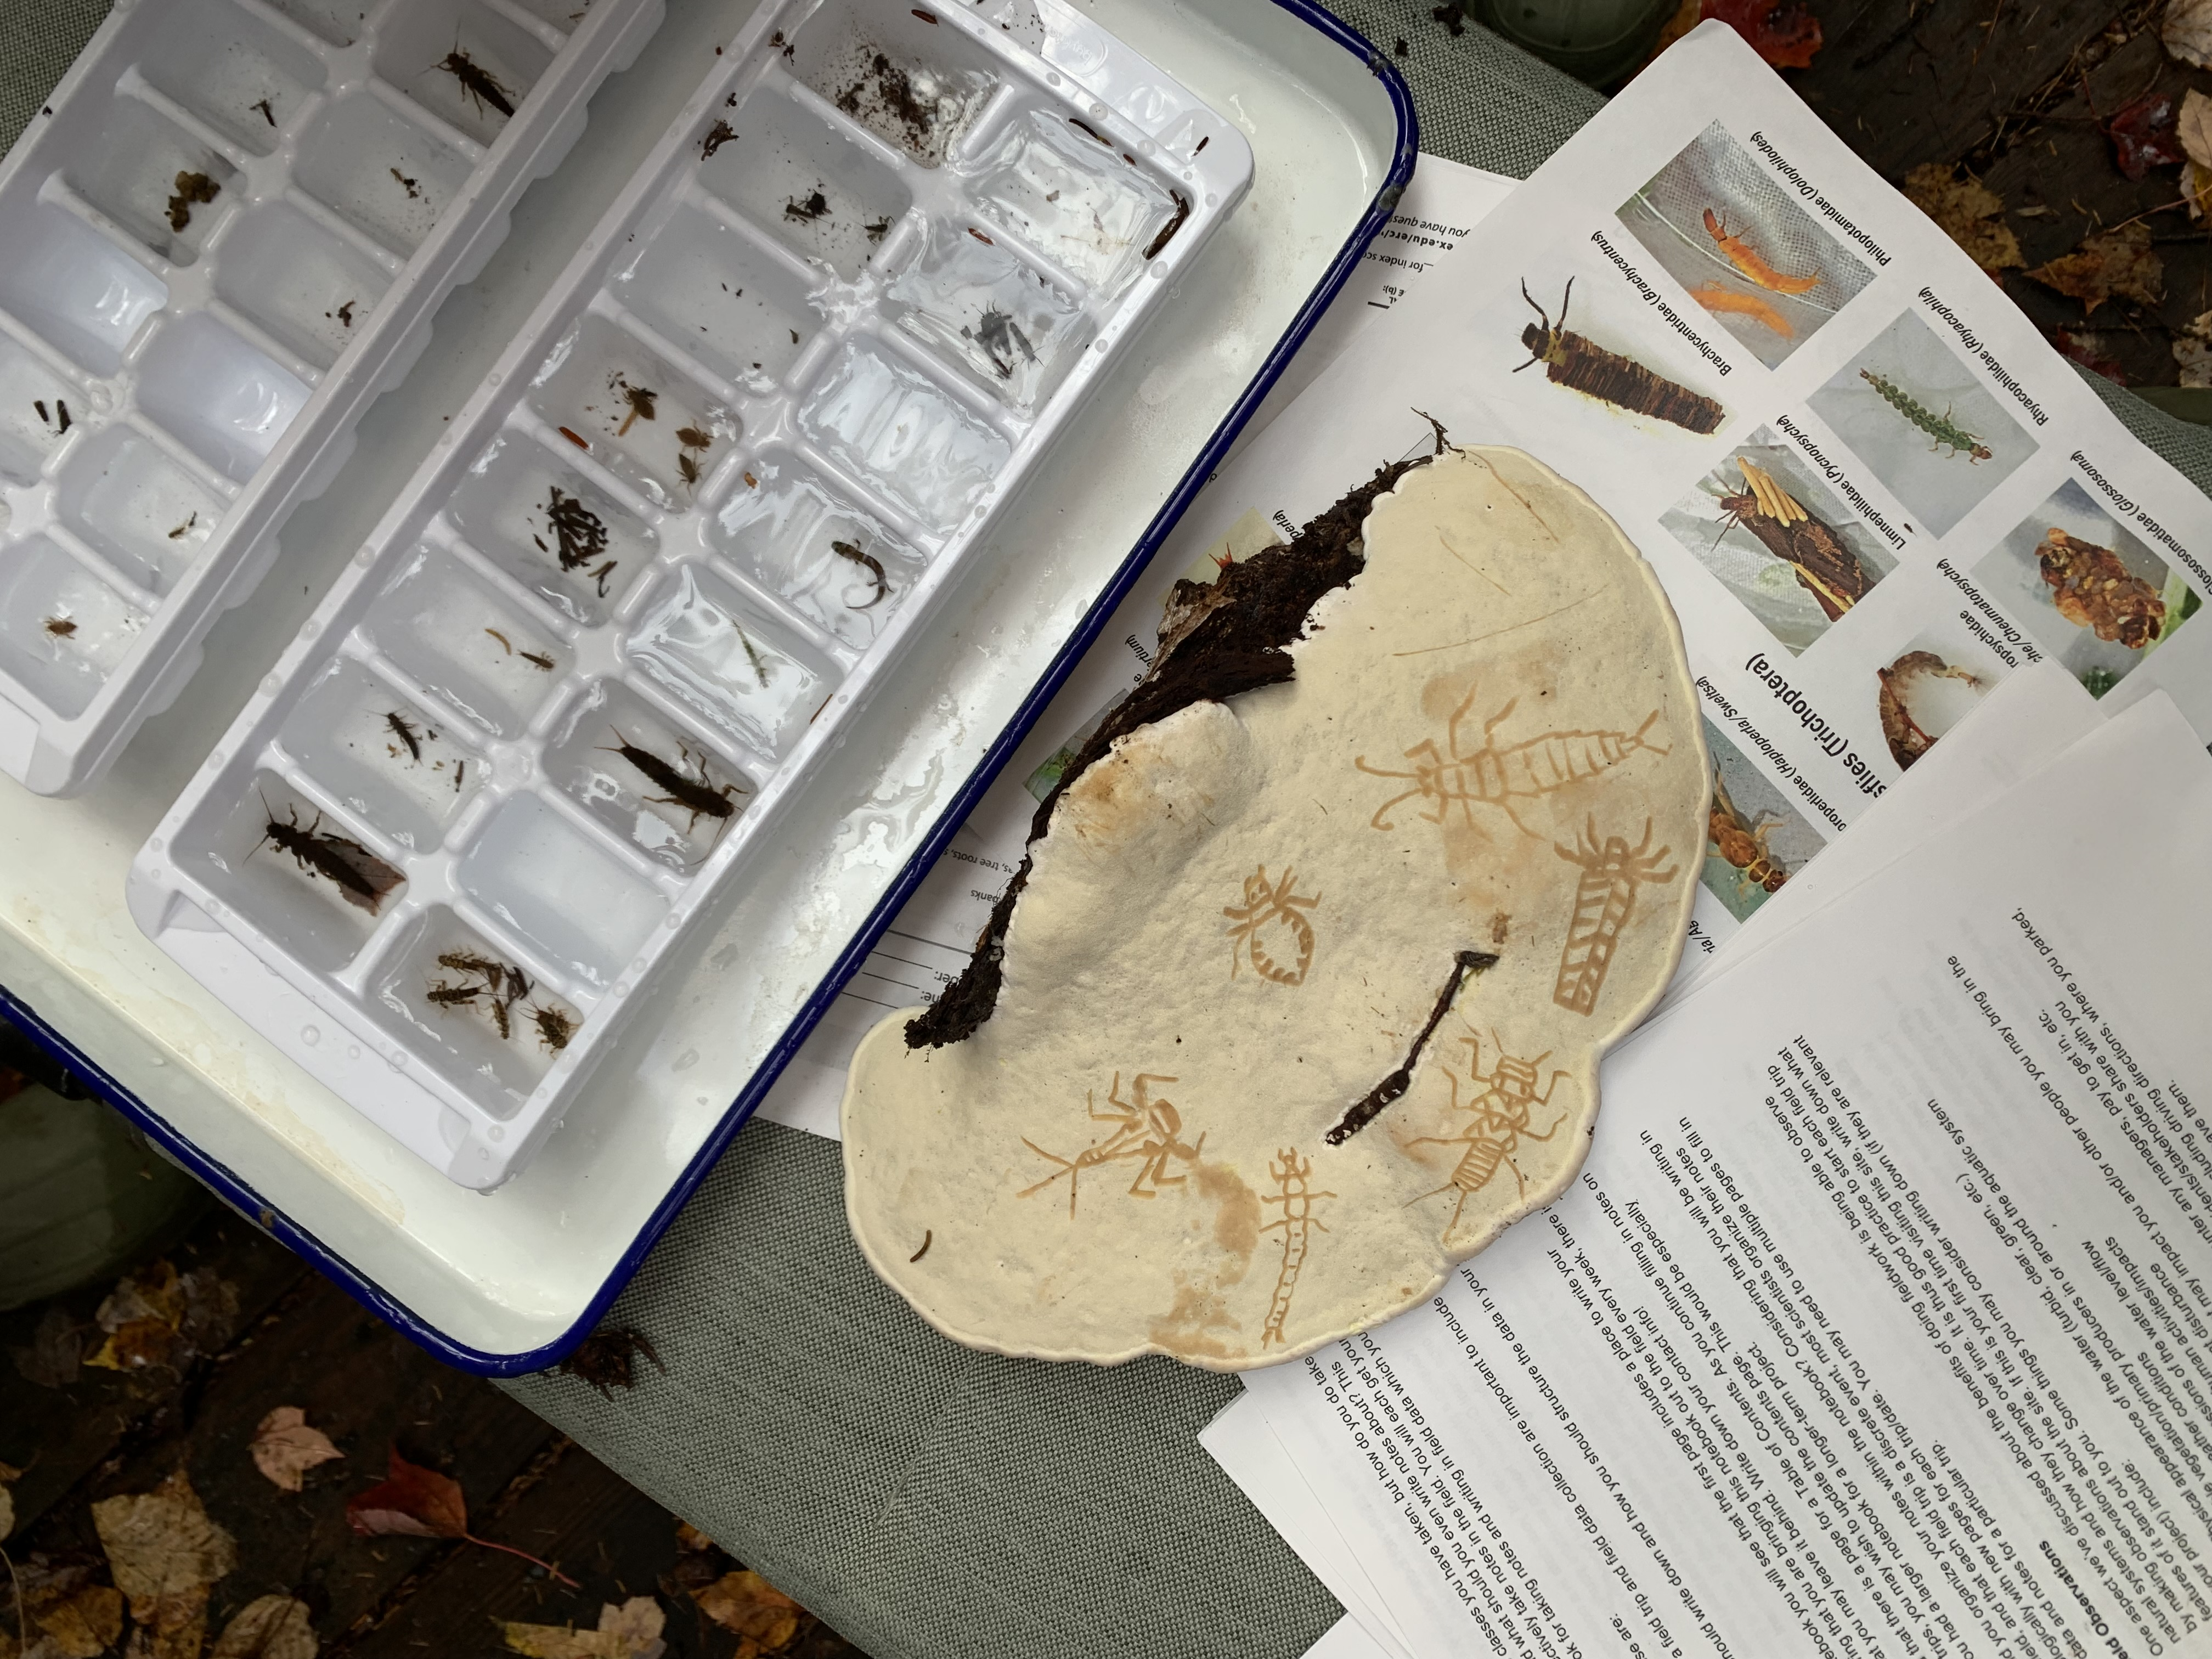
\includegraphics[width=0.32\textwidth,height=\textheight]{/Users/emilypower/Desktop/BIOL_1007A/Images/IMG_3101.jpeg}
\end{itemize}

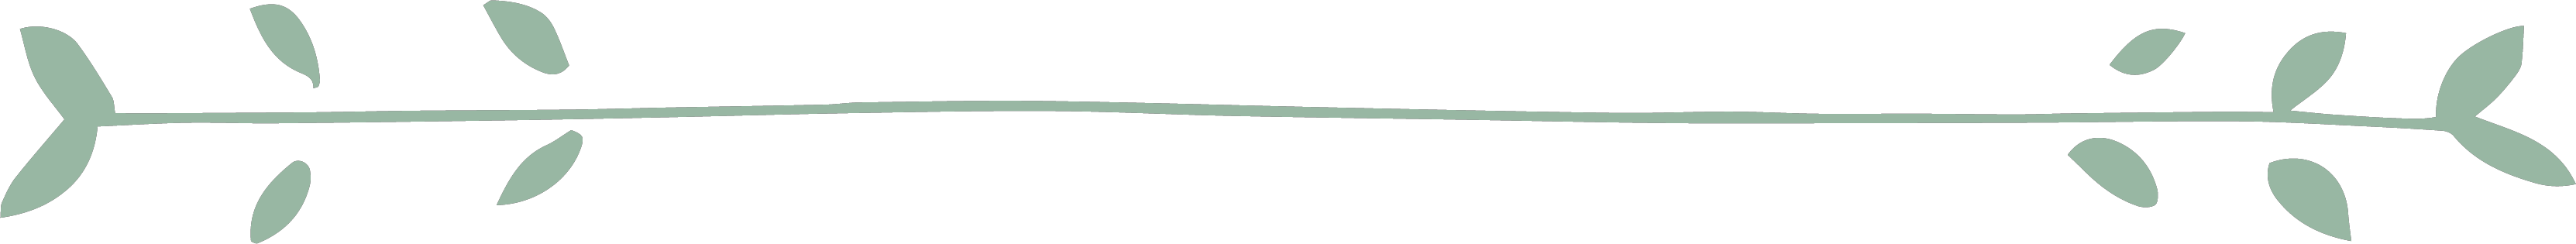
\includegraphics{/Users/emilypower/Desktop/BIOL_1007A/Images/Page_Break_Graphic_D2460FF10315A.png}

\hypertarget{this-j-term-i-decided-to-reproduce-the-figures-that-i-originally-generated-in-microsoft-excel-on-benthic-invertebrate-assemblages.-heres-what-they-looked-like-in-excel-apologies-for-the-poor-image-quality}{%
\paragraph{This J term, I decided to reproduce the figures that I
originally generated in Microsoft Excel on benthic invertebrate
assemblages. Here's what they looked like in Excel (apologies for the
poor image
quality!):}\label{this-j-term-i-decided-to-reproduce-the-figures-that-i-originally-generated-in-microsoft-excel-on-benthic-invertebrate-assemblages.-heres-what-they-looked-like-in-excel-apologies-for-the-poor-image-quality}}

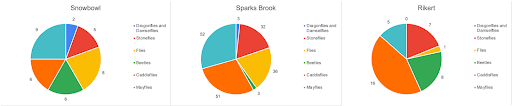
\includegraphics[width=1.5\textwidth,height=\textheight]{/Users/emilypower/Desktop/BIOL_1007A/Images/unnamed.png}

\begin{itemize}
\tightlist
\item
  \emph{Each figure displays benthic invertebrate counts categorized by
  taxonomic order across all three sampling sites.}
\end{itemize}

Generating these pie charts required a lot of data manipulation in Excel
prior to the actual chart creation. I also had to create each of them
separately. \textbf{I wanted to see if I could do that data manipulation
in R to reduce potential for error along the way.} You can see my
workflow below:

\begin{Shaded}
\begin{Highlighting}[]
\CommentTok{\# load packages}
\FunctionTok{library}\NormalTok{(dplyr)}
\end{Highlighting}
\end{Shaded}

\begin{verbatim}
## 
## Attaching package: 'dplyr'
\end{verbatim}

\begin{verbatim}
## The following objects are masked from 'package:stats':
## 
##     filter, lag
\end{verbatim}

\begin{verbatim}
## The following objects are masked from 'package:base':
## 
##     intersect, setdiff, setequal, union
\end{verbatim}

\begin{Shaded}
\begin{Highlighting}[]
\FunctionTok{library}\NormalTok{(ggplot2)}
\FunctionTok{library}\NormalTok{(ggthemes)}

\CommentTok{\# load data}
\NormalTok{raw\_insect\_data }\OtherTok{\textless{}{-}} \FunctionTok{read.table}\NormalTok{(}\AttributeTok{file =} \StringTok{"/Users/emilypower/Desktop/BIOL\_1007A/Data/BIOL 0304a Ski{-}Stream Data.csv"}\NormalTok{, }\AttributeTok{header =} \ConstantTok{TRUE}\NormalTok{, }\AttributeTok{sep=}\StringTok{","}\NormalTok{)}
\FunctionTok{glimpse}\NormalTok{(raw\_insect\_data)}
\end{Highlighting}
\end{Shaded}

\begin{verbatim}
## Rows: 78
## Columns: 12
## $ Location <chr> "Snowbowl", "Snowbowl", "Snowbowl", "Snowbowl", "Snowbowl", "~
## $ Species  <chr> "Gomphidae", "Leuctridae", "Chloroperlidae", "Chironomidae", ~
## $ Order    <chr> "Odonata", "Plecoptera", "Plecoptera", "Diptera", "Plecoptera~
## $ Count    <int> 1, 1, 1, 1, 1, 2, 1, 3, 2, 3, 3, 1, 4, 1, 1, 2, 1, 2, 1, 1, 2~
## $ X        <lgl> NA, NA, NA, NA, NA, NA, NA, NA, NA, NA, NA, NA, NA, NA, NA, N~
## $ X.1      <lgl> NA, NA, NA, NA, NA, NA, NA, NA, NA, NA, NA, NA, NA, NA, NA, N~
## $ X.2      <lgl> NA, NA, NA, NA, NA, NA, NA, NA, NA, NA, NA, NA, NA, NA, NA, N~
## $ X.3      <lgl> NA, NA, NA, NA, NA, NA, NA, NA, NA, NA, NA, NA, NA, NA, NA, N~
## $ X.4      <lgl> NA, NA, NA, NA, NA, NA, NA, NA, NA, NA, NA, NA, NA, NA, NA, N~
## $ X.5      <lgl> NA, NA, NA, NA, NA, NA, NA, NA, NA, NA, NA, NA, NA, NA, NA, N~
## $ X.6      <lgl> NA, NA, NA, NA, NA, NA, NA, NA, NA, NA, NA, NA, NA, NA, NA, N~
## $ X.7      <lgl> NA, NA, NA, NA, NA, NA, NA, NA, NA, NA, NA, NA, NA, NA, NA, N~
\end{verbatim}

\begin{Shaded}
\begin{Highlighting}[]
\FunctionTok{head}\NormalTok{(raw\_insect\_data)}
\end{Highlighting}
\end{Shaded}

\begin{verbatim}
##   Location                      Species      Order Count  X X.1 X.2 X.3 X.4 X.5
## 1 Snowbowl                    Gomphidae    Odonata     1 NA  NA  NA  NA  NA  NA
## 2 Snowbowl                   Leuctridae Plecoptera     1 NA  NA  NA  NA  NA  NA
## 3 Snowbowl               Chloroperlidae Plecoptera     1 NA  NA  NA  NA  NA  NA
## 4 Snowbowl                 Chironomidae    Diptera     1 NA  NA  NA  NA  NA  NA
## 5 Snowbowl                Peltoperlidae Plecoptera     1 NA  NA  NA  NA  NA  NA
## 6 Snowbowl Unknown (mayfly or stonefly)       <NA>     2 NA  NA  NA  NA  NA  NA
##   X.6 X.7
## 1  NA  NA
## 2  NA  NA
## 3  NA  NA
## 4  NA  NA
## 5  NA  NA
## 6  NA  NA
\end{verbatim}

\begin{Shaded}
\begin{Highlighting}[]
\CommentTok{\# clean up data}
\NormalTok{insect\_data }\OtherTok{\textless{}{-}}\NormalTok{ raw\_insect\_data[}\FunctionTok{complete.cases}\NormalTok{(raw\_insect\_data[,}\DecValTok{3}\NormalTok{]),] }\SpecialCharTok{\%\textgreater{}\%}  \CommentTok{\# remove counts with unknown taxonomic orders}
  \FunctionTok{group\_by}\NormalTok{(Location, Order) }\SpecialCharTok{\%\textgreater{}\%}  \CommentTok{\# group data by taxonomic order within each sampling location}
  \FunctionTok{summarize}\NormalTok{(}\AttributeTok{countSum=}\FunctionTok{sum}\NormalTok{(Count)) }\SpecialCharTok{\%\textgreater{}\%}  \CommentTok{\# summarize counts by order within each sampling location }
  \FunctionTok{mutate}\NormalTok{(}\AttributeTok{freq =}\NormalTok{ scales}\SpecialCharTok{::}\FunctionTok{label\_percent}\NormalTok{()(countSum }\SpecialCharTok{/} \FunctionTok{sum}\NormalTok{(countSum)))  }\CommentTok{\# adds a column (\textquotesingle{}freq\textquotesingle{}) that represents the percentage of each count within the total counts of a sampling site (contains values generated by dividing each countSum by the summary of countSum and converting the resulting decimal to a percentage)}
\end{Highlighting}
\end{Shaded}

\begin{verbatim}
## `summarise()` has grouped output by 'Location'. You can override using the
## `.groups` argument.
\end{verbatim}

\begin{Shaded}
\begin{Highlighting}[]
\NormalTok{insect\_data}
\end{Highlighting}
\end{Shaded}

\begin{verbatim}
## # A tibble: 17 x 4
## # Groups:   Location [3]
##    Location     Order         countSum freq  
##    <chr>        <chr>            <int> <chr> 
##  1 Rikert       Coleoptera           8 18.2% 
##  2 Rikert       Diptera              8 18.2% 
##  3 Rikert       Ephemeroptera        5 11.4% 
##  4 Rikert       Plecoptera           7 15.9% 
##  5 Rikert       Trichoptera         16 36.4% 
##  6 Snowbowl     Coleoptera           6 16.7% 
##  7 Snowbowl     Diptera              8 22.2% 
##  8 Snowbowl     Ephemeroptera        9 25.0% 
##  9 Snowbowl     Odonata              2 5.6%  
## 10 Snowbowl     Plecoptera           5 13.9% 
## 11 Snowbowl     Trichoptera          6 16.7% 
## 12 Sparks Brook Coleoptera           3 1.57% 
## 13 Sparks Brook Diptera             39 20.42%
## 14 Sparks Brook Ephemeroptera       52 27.23%
## 15 Sparks Brook Odonata              3 1.57% 
## 16 Sparks Brook Plecoptera          43 22.51%
## 17 Sparks Brook Trichoptera         51 26.70%
\end{verbatim}

I chose to use the \texttt{mutate()} function (above) because I couldn't
facet wrap three pie charts together with different sample sizes.
However\ldots{}

\textbf{Here's where I ran into an issue.} I tried to make a pie chart
using \texttt{insect\_data} but when I facet wrapped the three sampling
sites together, it looked like this:

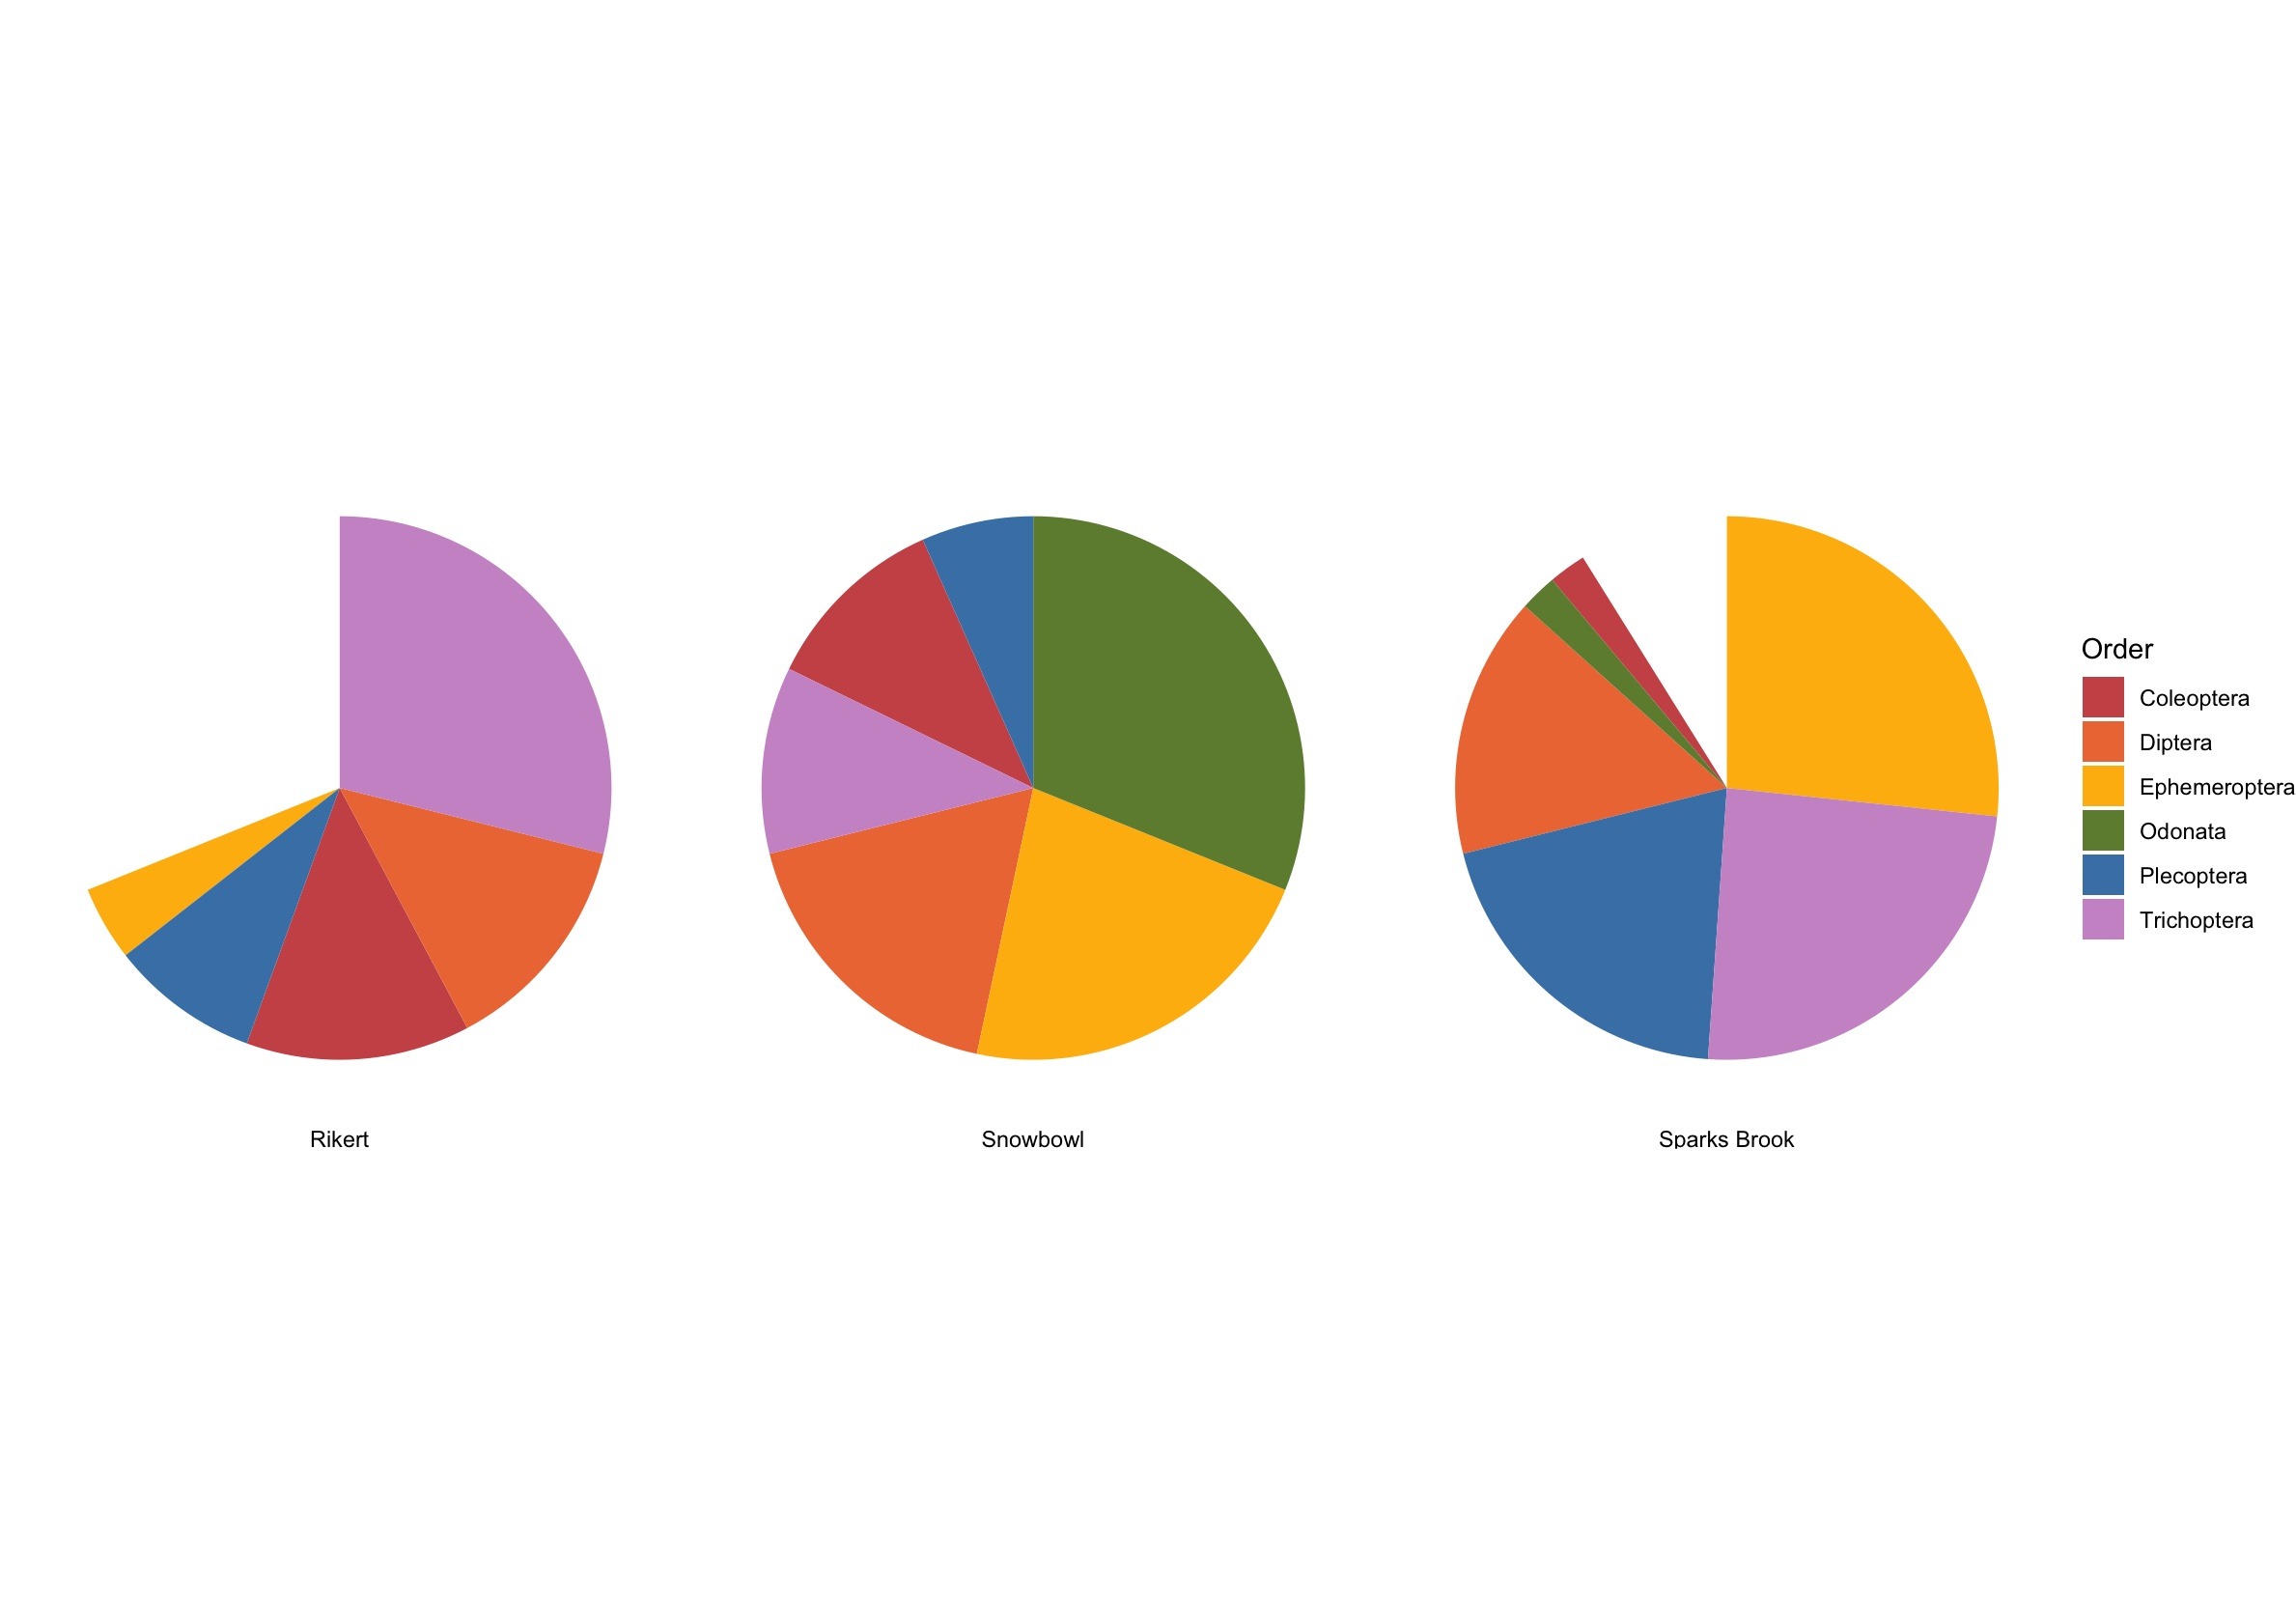
\includegraphics{/Users/emilypower/Desktop/BIOL_1007A/Images/pie_chart_error copy.jpg}

I think the issue was that I was using \texttt{freq} percentages, a
character value, instead of a numeric value, to create the slices of the
pie chart. To fix this, I found a way to add a column to my
\texttt{insect\_data} that included the frequency values without the
percentage sign. This new column (\texttt{freq\_numeric}) contains
numeric values.

\begin{Shaded}
\begin{Highlighting}[]
\NormalTok{new\_freq }\OtherTok{\textless{}{-}} \FunctionTok{as.numeric}\NormalTok{(}\FunctionTok{sub}\NormalTok{(}\StringTok{"\%"}\NormalTok{, }\StringTok{""}\NormalTok{, insect\_data}\SpecialCharTok{$}\NormalTok{freq))  }\CommentTok{\# create new variable that removes the percentage sign from freq values}
\NormalTok{final\_insect\_data }\OtherTok{\textless{}{-}} \FunctionTok{cbind}\NormalTok{(insect\_data, new\_freq)  }\CommentTok{\# add new variable to insect\_data}
\end{Highlighting}
\end{Shaded}

\begin{verbatim}
## New names:
## * `` -> `...5`
\end{verbatim}

\begin{Shaded}
\begin{Highlighting}[]
\NormalTok{final\_insect\_data }\OtherTok{\textless{}{-}} \FunctionTok{rename}\NormalTok{(final\_insect\_data, }\AttributeTok{freq\_numeric =}\NormalTok{ ...}\DecValTok{5}\NormalTok{)  }\CommentTok{\# name column \textasciigrave{}freq\_numeric\textasciigrave{}}
\FunctionTok{head}\NormalTok{(final\_insect\_data)}
\end{Highlighting}
\end{Shaded}

\begin{verbatim}
## # A tibble: 6 x 5
## # Groups:   Location [2]
##   Location Order         countSum freq  freq_numeric
##   <chr>    <chr>            <int> <chr>        <dbl>
## 1 Rikert   Coleoptera           8 18.2%         18.2
## 2 Rikert   Diptera              8 18.2%         18.2
## 3 Rikert   Ephemeroptera        5 11.4%         11.4
## 4 Rikert   Plecoptera           7 15.9%         15.9
## 5 Rikert   Trichoptera         16 36.4%         36.4
## 6 Snowbowl Coleoptera           6 16.7%         16.7
\end{verbatim}

\hypertarget{calling-the-freq_numeric-column-when-creating-my-pie-charts-worked}{%
\paragraph{\texorpdfstring{Calling the \texttt{freq\_numeric} column
when creating my pie charts
worked!}{Calling the freq\_numeric column when creating my pie charts worked!}}\label{calling-the-freq_numeric-column-when-creating-my-pie-charts-worked}}

\begin{Shaded}
\begin{Highlighting}[]
\CommentTok{\# generate chart}
\NormalTok{chart }\OtherTok{\textless{}{-}}\NormalTok{ final\_insect\_data }\SpecialCharTok{\%\textgreater{}\%}  \CommentTok{\# create chart from insect data}
  \FunctionTok{ggplot}\NormalTok{(}\AttributeTok{mapping =} \FunctionTok{aes}\NormalTok{(}\AttributeTok{x=}\StringTok{""}\NormalTok{, }\AttributeTok{y=}\NormalTok{freq\_numeric, }\AttributeTok{fill=}\NormalTok{Order)) }\SpecialCharTok{+}  \CommentTok{\# set y as insect count and fill as insect order}
  \FunctionTok{geom\_bar}\NormalTok{(}\AttributeTok{stat =} \StringTok{"identity"}\NormalTok{, }\AttributeTok{width=}\DecValTok{1}\NormalTok{) }\SpecialCharTok{+}  \CommentTok{\# create bar chart}
  \FunctionTok{coord\_polar}\NormalTok{(}\StringTok{"y"}\NormalTok{, }\AttributeTok{start=}\DecValTok{0}\NormalTok{) }\SpecialCharTok{+}  \CommentTok{\# make pie chart from bar chart}
  \FunctionTok{scale\_fill\_manual}\NormalTok{(}\AttributeTok{values =} \FunctionTok{c}\NormalTok{(}\StringTok{"indianred3"}\NormalTok{, }\StringTok{"sienna2"}\NormalTok{, }\StringTok{"darkgoldenrod1"}\NormalTok{, }\StringTok{"darkolivegreen4"}\NormalTok{, }\StringTok{"steelblue"}\NormalTok{, }\StringTok{"plum3"}\NormalTok{)) }\SpecialCharTok{+}  \CommentTok{\# set fill colors}
  \FunctionTok{theme\_void}\NormalTok{() }\SpecialCharTok{+}  \CommentTok{\# set chart theme}
  \FunctionTok{theme}\NormalTok{(}\AttributeTok{legend.position =} \StringTok{"right"}\NormalTok{) }\SpecialCharTok{+}  \CommentTok{\# add legend}
  \FunctionTok{facet\_wrap}\NormalTok{(}\SpecialCharTok{\textasciitilde{}}\NormalTok{Location, }\AttributeTok{ncol=}\DecValTok{3}\NormalTok{, }\AttributeTok{strip.position=}\StringTok{"bottom"}\NormalTok{)  }\CommentTok{\# separate pie charts by sampling location}
\end{Highlighting}
\end{Shaded}

\textbf{Here's the final product!}

\begin{Shaded}
\begin{Highlighting}[]
\NormalTok{chart}
\end{Highlighting}
\end{Shaded}

\includegraphics{Final_Assignment_files/figure-latex/unnamed-chunk-4-1.pdf}

\textbf{Fig. 1} Benthic macroinvertebrate abundances categorized by
taxonomic order from three different stream sites in Vermont. Snowbowl
and Rikert streams were sampled on the same day, Sparks Brook one week
later. Samples were taken by students using a Surber sampler and
identified using a taxonomic key.

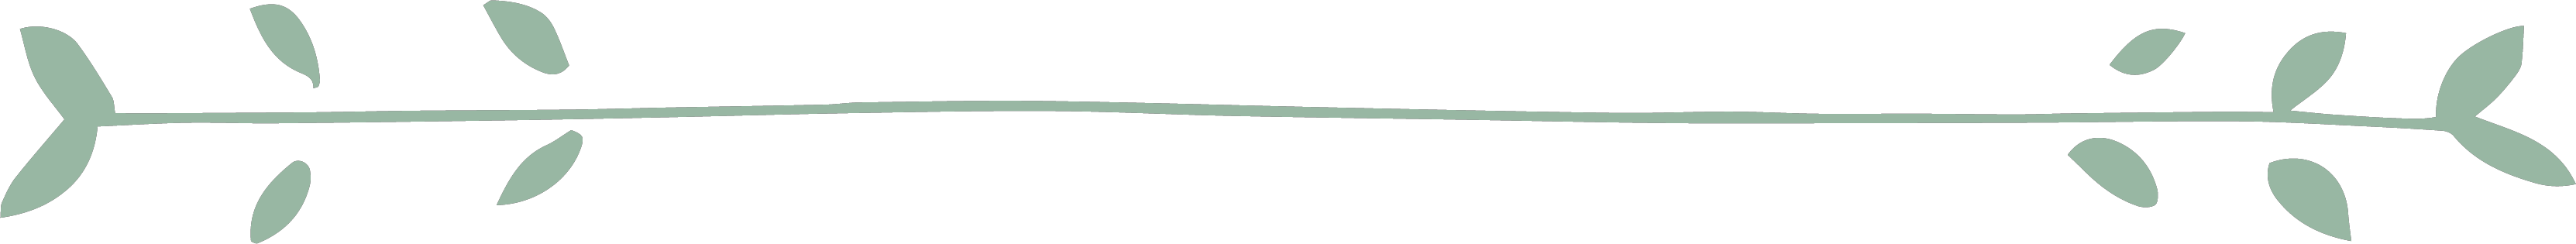
\includegraphics{/Users/emilypower/Desktop/BIOL_1007A/Images/Page_Break_Graphic_D2460FF10315A.png}

With a little extra curiosity, I wanted to see if there was significant
variation in benthic invertebrate assemblages between stream sites. To
do so, I decided to re purpose the ANOVA function I created in
\href{/Users/emilypower/Desktop/BIOL_1007A/Weekly\%20Assignments/Weekly_Assignment_2.html}{Weekly
Assignment 2}. I chose to compare insect taxonomic order assemblages
across streams, as opposed to raw counts, because we spent different
amounts of time sampling at each stream site. Thus, the counts were more
reflective of the time invested than the actual stream composition.

\begin{Shaded}
\begin{Highlighting}[]
\DocumentationTok{\#\#\#\#\#\#\#\#\#\#\#\#\#\#\#\#\#\#\#\#\#\#\#\#\#\#\#\#\#\#\#\#\#\#\#\#\#\#\#\#\#\#\#\#\#\#\#\#\#\#\#\#\#\#\#\#\#\#\#\#\#\#\#\#\#\#\#\#\#\#\#\#}
\CommentTok{\# FUNCTION: ANOVA\_function}
\CommentTok{\# returns the p{-}value of an ANOVA summary table}
\CommentTok{\# input: a data frame}
\CommentTok{\# outputs: p{-}value}
\CommentTok{\#{-}{-}{-}{-}{-}{-}{-}{-}{-}{-}{-}{-}{-}{-}{-}{-}{-}{-}{-}{-}{-}{-}{-}{-}{-}{-}{-}{-}{-}{-}{-}{-}{-}{-}{-}{-}{-}{-}{-}{-}{-}{-}{-}{-}{-}{-}{-}{-}{-}{-}{-}{-}{-}{-}{-}{-}{-}{-}{-}{-}{-}{-}{-}{-}{-}{-}{-}{-}{-}{-}{-}}
\NormalTok{ANOVA\_function }\OtherTok{\textless{}{-}} \ControlFlowTok{function}\NormalTok{(}\AttributeTok{df=}\NormalTok{final\_insect\_data)\{}
\NormalTok{  test }\OtherTok{\textless{}{-}} \FunctionTok{aov}\NormalTok{(freq\_numeric }\SpecialCharTok{\textasciitilde{}}\NormalTok{ Location, }\AttributeTok{data=}\NormalTok{df)  }\CommentTok{\# is there statistically significant variation in insect assemblages between stream sites?}
\NormalTok{  test\_summary }\OtherTok{\textless{}{-}} \FunctionTok{summary}\NormalTok{(test)  }\CommentTok{\# makes test summary}
\NormalTok{  p\_value }\OtherTok{\textless{}{-}}\NormalTok{ test\_summary[[}\DecValTok{1}\NormalTok{]][[}\StringTok{"Pr(\textgreater{}F)"}\NormalTok{]][}\DecValTok{1}\NormalTok{]  }\CommentTok{\# pulls p value from test summary}
  \FunctionTok{return}\NormalTok{(p\_value)  }\CommentTok{\# returns p value}
\NormalTok{\}}

\NormalTok{insect\_pValue }\OtherTok{\textless{}{-}} \FunctionTok{ANOVA\_function}\NormalTok{()}
\NormalTok{insect\_pValue}
\end{Highlighting}
\end{Shaded}

\begin{verbatim}
## [1] 0.8126263
\end{verbatim}

If the code above is set up correctly, the high p-value indicates that
stream location had \textbf{no significant impact on benthic
invertebrate assemblages when considering taxonomic order.}

\end{document}
